%%%%%%%%%%%%%%%%%%%%%%%%%%%%%% -*- Mode: Latex -*- %%%%%%%%%%%%%%%%%%%%%%%%%%%%
%% main.tex<fourier_decomp> -- 
%% Last Modified On: Thu Apr 13 16:15:17 2023 (+0200)
%%%%%%%%%%%%%%%%%%%%%%%%%%%%%%%%%%%%%%%%%%%%%%%%%%%%%%%%%%%%%%%%%%%%%%%%%%%%%%%

\documentclass{zamarep}

% Useful LaTeX packages
\usepackage{mathtools}
\usepackage{mathcalbd} % for \pol macro

\usepackage[colorlinks]{hyperref} % should be loaded last
\usepackage{cleveref}  % should be loaded last last

\title{Towards Verifiable TFHE}
\subtitle{Proving Correct Execution of the External Product Using PLONK}

\author[MW]{Michael Walter}

\date{April 13, 2023}

\titlegraphic[credit={Erik Karits}]{%
  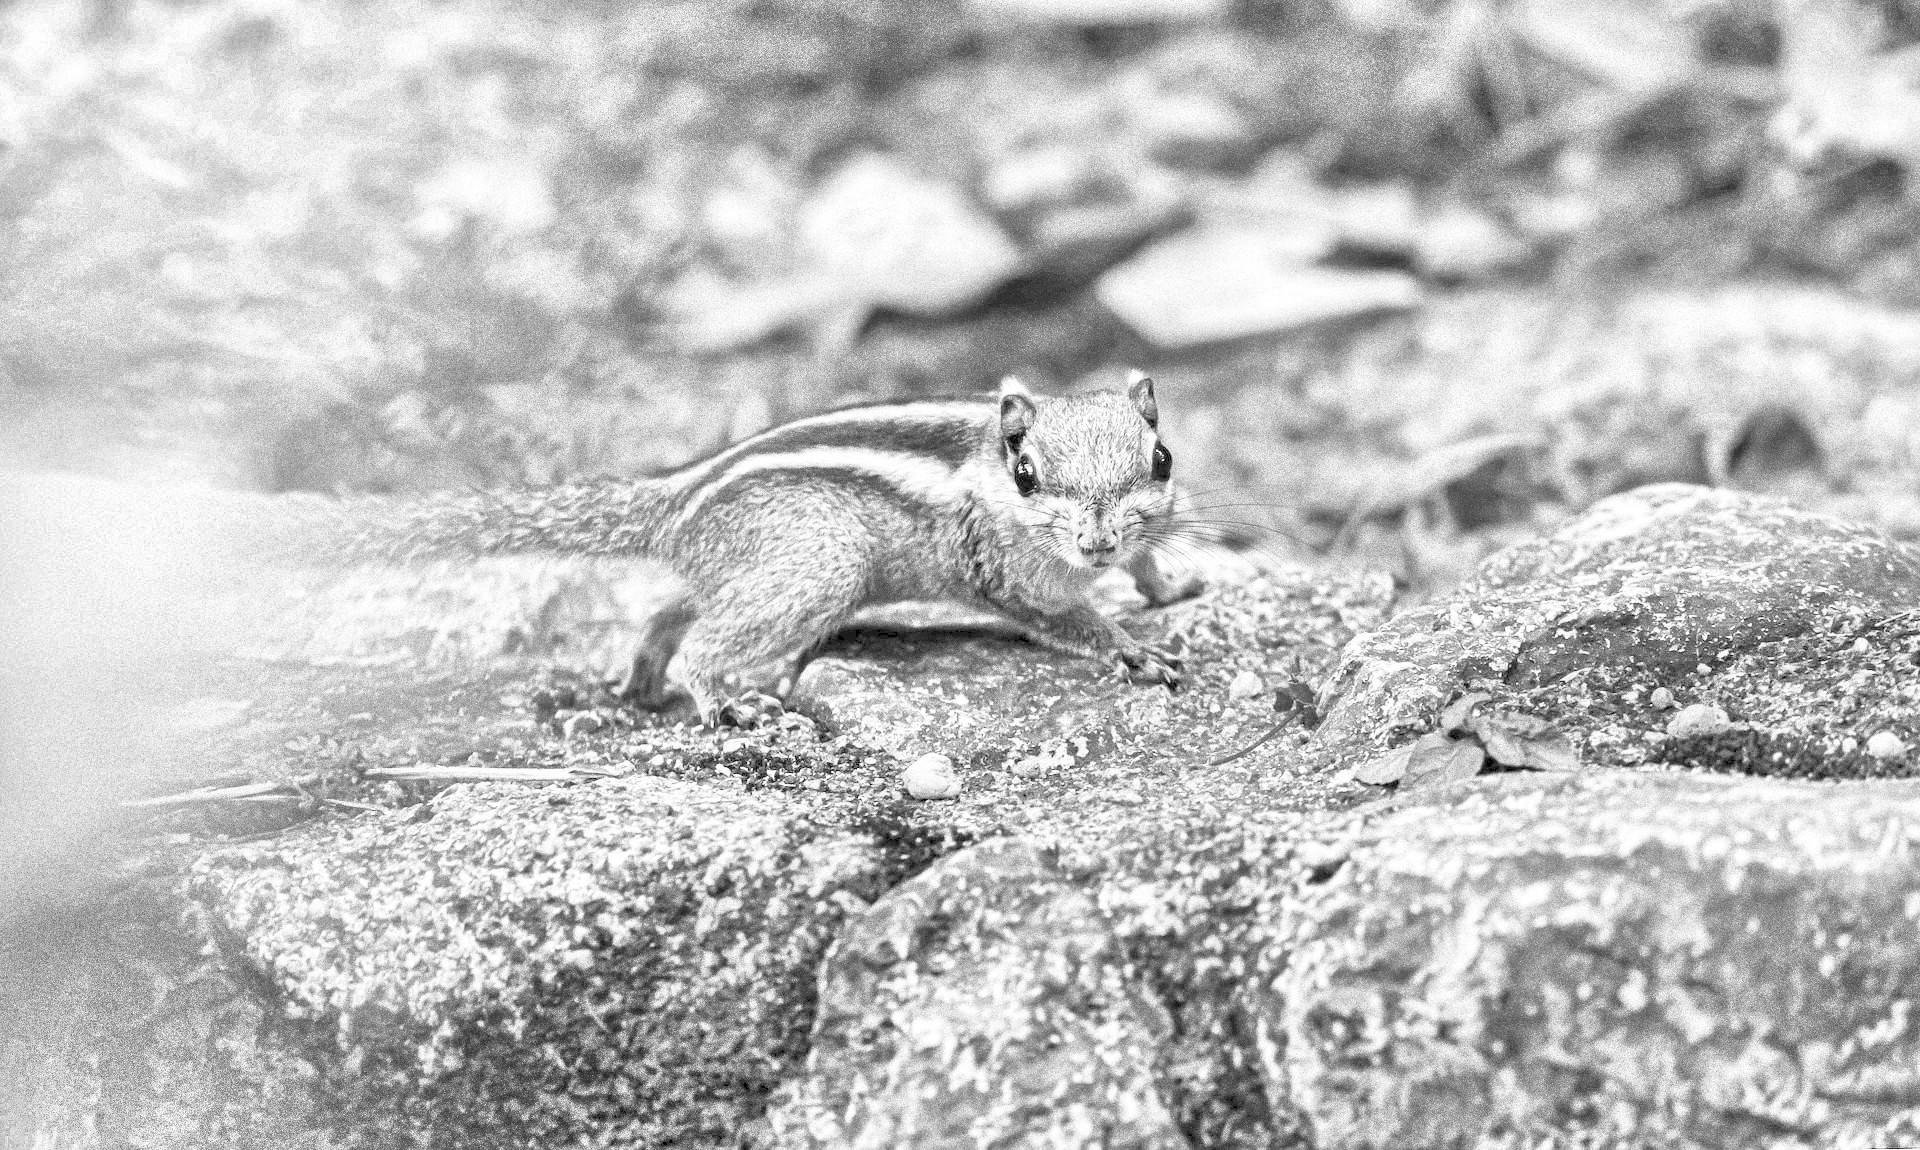
\includegraphics{erik-karits-Ivy_nqt6gTc-unsplash}}


% --- Macros
% \newcommand{\ints}{\mathds{Z}}
% \newcommand{\reals}{\mathds{R}}
% \newcommand{\torus}{\mathds{T}}
% \newcommand*{\pol}{\mathcalbd}
% \newcommand*{\SQ}{\mathit{S\!Q}}
\newcommand{\field}{\mathbb{F}}

\begin{document}

\maketitle


%%%%%%%%%%%%%%%%%%%%%%%%%%%%%%%%%%%%%%%%%%%%%%%%%%%%%%%%%%%%%%%%%%%%%%%%%%%%%%% 
\section{Introduction}\label{sec:introduction}
%%%%%%%%%%%%%%%%%%%%%%%%%%%%%%%%%%%%%%%%%%%%%%%%%%%%%%%%%%%%%%%%%%%%%%%%%%%%%%% 

FHE is inherently not IND-CCA2 secure, i.e.\ a malicious adversary or server might tamper with ciphertexts and obtain information about the secret key or data of the client by observing its behaviour upon decryption. A possible solution is to require the server to prove to a client that a ciphertext is the result of a homomorphic computation using a SNARK (Succinct Non-interactive Argument of Knowledge).

One of the goals of Q1 2023 was to prototype a specific SNARK and prove the correct execution of TFHE's external product using it. This report documents this effort. There is a wide range of SNARK candidates to choose from and in a previous step of this project, the combination of PLONK and FRI was identified as promising approach for TFHE. See the notion page\footnote{\url{https://www.notion.so/zamaai/SNARKs-bd3b32818e0146a597ad1aaeebb3ca4c}} for further details and below for a description.

Before describing our implementation, we remark a subtlety of SNARKs in the FHE setting: the general idea of FHE is to outsource computation and SNARKs are a suitable candidate in this setting because verification time is typically sublinear in the circuit size. However, they require a setup/preprocessing that is linear in the circuit size and produce some ``compressed'' information about the circuit for the verifier. An advantage of our approach based on FRI is that the setup is entirely transparent and can be performed by anyone. But still it is not clear in our setting which party should perform the preprocessing. If the client performs it itself, this might defeat the purpose of using FHE in the first place since a linear preprocessing is similarly expensive as performing the computation in the first place. So this approach is only useful if the same circuit is applied multiple times, such that the preprocessing effort of the client can be amortized over many computations. An example could be database or ML queries. Another approach could be to let the server perform the preprocessing, but this begs the question how the client can check the preprocessing without spending too much computational effort. A plausible approach could require the server to commit to the output of the preprocessing by, e.g., uploading the verifier input (or the hash value thereif) to a blockchain. Since anyone can perform the preprocessing, anyone can also re-run it and check the server's honesty. So a cheating server runs a very high risk of potentially being caught by someone (not necessarily a client). We envision this application and for this reason we treat the preprocessing in our implementation as part of the proof. 


\section{Description of Algorithms}
\label{sec:desc}

For ease of prototyping the implementation was written in Sage\footnote{\url{https://www.sagemath.org/}}. The obvious downside is that a lot of the code is in Python, which means it is relatively inefficient. Our implementation consists of three files, mirroring the different parts of the SNARK:
\begin{itemize}
\item \texttt{poly\_fri.sage}: the Polynomial Commitment Scheme (PCS) based on FRI
\item \texttt{plonk.sage}: the PLONK arithmetization
\item \texttt{circuit.sage}: some code to build circuits and generate the data required by PLONK.
\end{itemize}

Roughly speaking, PLONK encodes a computation trace of a circuit into a polynomial and then the PCS is used to prove statements about this polynomial that ensure correct execution. In the following we give a high level description of the algorithms and our implementation thereof. For further details we refer to the MOOC on Zero Knowledge Proofs (2023)\footnote{\url{https://zk-learning.org/}}, in particular Lecture 5 on PLONK and Lecture 8 on FRI.


\subsection{FRI-based Polynomial Commitment Scheme}
\label{sec:fri}

A PCS allows a prover to commit to a polynomial of bounded degree. Then, a verifier, given such a commitment, may query the prover for evaluations of the committed polynomial at arbitrary points. The scheme ensures that the query responses of the prover are consistent with the initial commitment.

In FRI\footnote{Technically, FRI is not a PCS, but a protocol to prove closeness to a Reed-Solomon code, but it can be turned into a PCS. So in this report, when we refer to FRI, we mean the PCS build from FRI.}, the commitment of a polynomial $f$ of degree $k$ is computed by turning it into a Reed-Solomon codeword of length $n = \beta \cdot k$ and committing to the codeword via a Merkle hash. In order to open $f$ at a point $r$ as $f(r) = v$, the prover shows that $f(x) - v = q(x) \cdot (x - r)$ by showing that $q(x)$ is close to a codeword. This is done by folding the codeword into smaller codewords using random linear combinations, until it is small enough to send the entire codeword. Each of these codewords is committed to using a Merkle hash and the verifier can check the correctness using openings of the Merkle hashes at random points. We denote these random points by \emph{samples}.

The parameter $\beta$ controls the trade-off between prover and verifier complexity (and proof size). Every verifier query (heuristically) provides about $\log \beta$ bits of security, so larger $\beta$ allows fewer queries at the same level of security, which reduces the proof size and verifier complexity. On the other hand, the complexity of the prover is dominated by computing RS codewords of size $n$, which costs $O(n \log n)$ operations. Since the size of the RS code $n$ grows linearly in $\beta$, the prover complexity grows super-linearly with $\beta$. In our prototype, we set $\beta = 4$.

\paragraph{A Note on Hashing}
For the PCS, hashing is required for two purposes: to compute Merkle hashes and in order to perform the Fiat-Shamir transform. The latter requires that the output of the hash function is a field element $\field_p$. If we use the same hash function for the Merkle hashes, then all the inputs to the hash function are also elements from $\field_p$. So it makes sense to use some arithemtic hash function $\{\field_p\}^* \mapsto \{\field_p \}^o$ for some length $o$. Note that for the Merkle hash we need to set $o$ large enough so that the hash function is collision resistant, i.e. $o \geq 2 \lambda / \log p$. Collision resistance is not required for Fiat-Shamir, so we may choose a different $o$ for Fiat-Shamir. In particular, $o=1$ is convenient, since the random coins of the verifier always yield a single field element. In our prototype implementation, we set $o = 1$ for both, even though our field is rather small --- we choose $p = 2^{64} - 2^{32} + 1$. 

There are different choices of arithmetic hash functions and we provide an ad-hoc implementation of Poseidon \cite{USENIX:GKRRS21}. However, this implementation is very slow and renders the prototype impractical even for small examples. Since an efficient hash function implementation was not the focus of this project, we instead use a toy hash function, which is sufficient for correctness, but provides no security guarantees. 

\subsection{PLONK Arithmetization}
\label{sec:plonk}
Given the evaluation trace of a circuit, i.e. the values of all inputs and wires, PLONK encodes the entire trace in a polynomial $T$. This encoding is done by setting the values of $T$ to be the values in the trace at powers of a $d$-th root of unity. Clearly, $d$ must be large enough to encode all value in the trace, so, roughly speaking, we have $d \geq 3 \lvert C \rvert$, where $\lvert C \rvert$ is the number of gates of the circuit. (Technically, we need to add the number of inputs since they need to be encoded as well.) Computing the polynomial $T$ can be done via an inverse NTT, so requires $O(d \log d)$.

Once the polynomial $T$ is computed, it is committed to using FRI, which requires to compute the corresponding codeword using, e.g. a forward NTT in $O(n \log n) = O(d \log d)$. Computing and committing to the polynomial $T$ are the two steps that dominate the complexity of the prover.

Then the verifier needs to ensure that it indeed encodes a correct execution by querying $T$. Four properties of $T$ need to be checked:
\begin{enumerate}
\item encoding of the inputs,
\item encoding of the outputs,
\item evaluation of gates,
\item the wiring between the gates.
\end{enumerate}
The first two are relatively straight-forward, while the latter two are more involved. For brevity, we will not go into further detail here and refer to the resources mentioned above. But we do remark here that the checks can be performed by a constant number of PCS queries to $T$ (or related polynomials).

Finally, we note that checking the evaluation of gates and the wiring requires some auxiliary polynomials. The verifier needs a commitment to these polynomials, which is computed during preprocessing. As stated in Section \ref{sec:introduction}, we compute these polynomials and their commitments during proof generation on the prover side and consider them part of the proof.

\subsection{Circuit Generation}
\label{sec:circuit}
Generating the information required by the PLONK arithmetization from a circuit by hand is tedious and error-prone, so we provide some additional code that allows to build circuits and automatically generate the trace and additional information (gate types, wiring, etc) from such circuits. Using this code, we build sub-circuits for more complex tasks like arithmetic in $\field_p[X]/(X^N + 1)$ and gadget decomposition required for the external product. We discuss these latter two operations in a little more detail since they dominate the size of the circuit.

\paragraph{Polynomial Multiplication}
In our first prototype, we implemented polynomial multiplication in a naive way using matrix multiplication. This means that the multiplication algorithm involves $N$ inner products, each of which requires $N$ multiplication and $N - 1$ addition gates. Since some of the terms need to be negated, about $N$ additional multiplication gates (with the constant $-1$) are required. All in all this results in about $2 \cdot N^2$ gates.

\paragraph{Gadget Decomposition}
Gadget decomposition with base $B$ decomposes a number into a vector of smaller numbers\footnote{For this prototype we only consider exact decomposition.} $a = \sum_{i = 0}^{\ell-1} a_i B^i$. Using signed decomposition, we may ensure that $\lvert a_i \rvert \leq B/2$. This operation $a \mapsto (a_i)_i$ is not easily implemented using arithmetic gates, but the inverse operation $(a_i)_i \mapsto a$ is. So in our implementation, we treat the $a_i$'s as part of the secret prover input, build the recombination circuit from it and require identity with the element to be decomposed. Note that equality constraints are essentially free in PLONK, so this only requires $2 \ell - 1 = 2 \cdot \log_B p - 1$ gates. It remains to prove that the $a_i$'s are indeed in $[-B/2, B/2]$. This can be done with a range check, i.e., for each $i$ we check that $\prod_{b = -B/2}^{B/2} (a_i - b) = 0$, which requires $2B + 1$ gates. Since this range check needs to be performed on all $a_i$, the overall number of gates for the range checks is $(2B + 1) \cdot \ell = (2B + 1) \cdot \log_B p $. Minimizing cost over the two operations we found $B = 4$ and $\ell = 32$ to provide the smallest circuit size. Note that it is still possible to prove gadget decomposition using a larger base $B$ at essentially the same cost by performing the range check itself using a gadget decomposition. This will reduce the number of terms in the inner product and thus might reduce overall circuit size. However, at this point this is not implemented in our prototype. PLONK also supports custom gates for operations that are frequently repeated. Gadget decomposition seems to be a natural candidate here, which we might consider in the future.

\section{Performance}

We report on some preliminary statistics and performance results here. As noted before, we set $p = 2^{64} - 2^{32} + 1$ and assume that the ciphertext modulus of TFHE is set to be the same prime. 

\paragraph{Circuit Size}
The way we currently implement the circuit for an external product requires for each polynomial in $\field_p[X]/(X^N + 1)$:
\begin{itemize}
\item $N \cdot ((2 \cdot \ell - 1) + \ell \cdot (2 \cdot B + 1))$ gates for gadget decomposition
\item about $\ell \cdot 2 \cdot N^2$ gates for polynomial multiplications
\item $N * (\ell - 1)$ gates for polynomial additions.
\end{itemize}
For example, if $N = 1024$, then the circuit for the external product has about $2^{26}$ gates, which means the degree of the polynomial the prover needs to handle is about $d \approx 2^{28}$ and the corresponding RS code has size $n = \beta d$. Recall that the prover runs in time $\Omega(n \log n)$, so, even ignoring constants, this is a computational load of at least $2^{35}$ (assuming $\beta = 4$) for just the external product. Note that this is only for a single polynomial of the ciphertext, so this needs to be repeated for each polynomial in the ciphertext. Luckily, the computation on the different polynomials is independent and thus we can prove them separately. 


\paragraph{Proof Size and Prover Performance for Small Instances}
Recall that our hash function does not provide any security and we did not spend much time trying to optimize the code, so our implementation is not capable of handling anything that resembles real-world instance. Still, to get a sense of what we may expect, we provide some rough performance numbers for instances that we were able to run.

We set the number of samples for the FRI protocol, i.e.\ the number of random points to open for each PCS opening, to be $32$, which, together with the blow-up factor $\beta=4$ should result in about 64 bits of security (assuming we use a secure hash function). We note though that the proof size (and verifier complexity) only depends linearly on the number of samples and does not significantly impact prover complexity, so this may be increased to achieve higher security levels.

For $N=2$ (circuit size $\approx 2^{10}$), the external product required about $2.5$ minutes on a mediocre laptop (Intel Core i5-5200U CPU @ 2.20GHz) and the proof contained about $2^{17}$ field elements, so about $2^{20}$ bytes, or $1$ MB. This may seem a lot for such a small instance, but we stress that the proof size is significantly more sensitive to the security level and the blow-up factor than the circuit size. In particular, the proof size grows as $O(\lambda \cdot \log^2 n)$, so only poly-logarithmically in the circuit size. Accordingly, for $N=4$ (circuit size $\approx 2.5 * 2^{10}$), the proof size only increased by about 13 percent, while the running time quadrupled to almost 10 minutes.

\section{Outlook}
\label{sec:outlook}

Here, we describe several ways forward towards an efficient prover for the external product.

\paragraph{Power of 2 Ciphertext Modulus}
So far we have assumed that the ciphertext modulus matches the SNARK modulus. However, note that most SNARKS require a field, i.e.\ a prime modulus, while we typically select a power of 2 modulus for TFHE. There are a couple of approaches that we may explore to prove the external product with power of 2 modulus. First, we may choose a large prime for the SNARK and emulate operations in $\mathbb{Z}_q$ (where $q$ is the ciphertext modulus). Some tricks that may speed this up are given in \cite{viand2023verifiable}, but this would still significantly increase the size of the circuit. Another approach could be to use a SNARK that natively can work with rings instead of fields. The only example we are aware of is given in \cite{EPRINT:GanNitSor21}. This has the drawback of requiring trusted setup (which essentially means the client has to run it) and only supporting a designated verifier, not public verifiability.

Given the current options, we believe the overall easiest and most performant solution is likely to change the ciphertext modulus of TFHE to match the SNARK modulus.

\paragraph{More Efficient Range Proofs via Plookup}
Recall that reducing the size of the circuit is crucial in order to reduce prover running time. One way of doing so is to perform the range checks more efficiently, using techniques like \cite{EPRINT:PFMBM22,EPRINT:GabWil20}.

\paragraph{Hyperplonk}
Note that even with smaller circuit size, the SNARK prover has a larger asymptotic complexity than the FHE evaluator, since it is superlinear in the circuit size. One way of improving prover time is a recent work \cite{EPRINT:CBBZ22}. In many ways it is similar to PLONK, but avoids the Fourier transforms (that introduce the large complexity) by moving from univariate polynomials to multivariate polynomials. This requires also modification of the PCS, since it also needs to handle multivariate polynomials. A technique for transforming a PCS for univariate polynomials into a PCS for multivariate polynomials is also given in the paper. Technically, the modified PCS based on FRI will still require super-linear time, so a different PCS might be required. 

\paragraph{Blind Rotation}
Proving the external product is only a stepping stone towards proving the correctness of the entire PBS. The next step will be to prove the blind rotation, which consists of a number of successive external products. The naive way of doing so would simply string together the circuits for each external product. This will blow up the circuit size by a linear factor and thus the prover complexity by a superlinear factor (unless using Hyperplonk). It might be possible to avoid this by using Incrementally Verifiable Computation \cite{TCC:Valiant08} based on recursive SNARKs. This can be made more efficient in terms of proof size and verifier complexity by using proof folding for PLONK \cite{sangria}.

% --- Bibliography
\bibliographystyle{alphaurl}
\bibliography{../../../cryptobib/abbrev1,../../../cryptobib/crypto,local}

\end{document}
